\section{Introduzione}
Nella secconda iterazione sono stati implementati la maggior parte dei casi d'uso: viene proposta 
un'analisi dettagliata al fine di specificare le seguenti informazioni:
\begin{itemize}
    \item \textbf{Attori:} vengono specificati quali attori sono coinvolti nel caso d'uso in analisi.
    \item \textbf{Precondizioni:} condizioni che devono necessariamente essere verificate per il corretto funzionamento del sistema nel caso d'uso in analisi. 
    \item \textbf{Postcondizioni:} condizioni che saranno verificate a seguito di un corretto funzionamento del sistema nel caso d'uso in analisi. 
    \item \textbf{Sequenza base:} riassume gli step base del caso d'uso in analisi.
    \item \textbf{Sequenza in caso di eccezioni:} specifica i casi d'eccezione possibili e a che passo della Base Sequence si viene riportati. 
\end{itemize}

Dopo aver analizzato nel dettaglio i casi d'uso si procede con la parte di Testing, 
quindi analisi statica e dinamica tramite Electron. (...)


\newpage

\section{Implementazione}
Di seguito sono elencati i casi d'uso implementati nel sistema WeMusic. Si offre, per ognuno, una breve descrizione dello stesso 
al fine di riassumere la sua funzionalità; inoltre è evidenziato il flow di esecuzione del sito e le varie alterntive che si propongono nel modello.
Infine, vengono specificate eventuali informazioni relative a precondizioni, post condizioni e trigger dello stesso, e le possibili eccezioni nel 
caso avvenga una esecuzione scorretta. 
Seguendo la modellazione proposta in seguito, i casi d'uso relativi all'Autenticazione sono stati completamente implementati, come anche 
la maggior parte di quelli facenti parte del gruppo Musica e Amici. 
\subparagraph{Bootstrap}
Per il frontend è stato utilizzato Bootstrap, un framework per frontend e web development semplice e veloce. 
Bootstrap include templates design basati su HTML e CSS per tipografia, forme, pulsanti, tabelle, navigazione, caroselli di 
immagini e molto altro, come anche plugin opzionali di JavaScript; è' molto semplice da usare e possiede un'alta 
compatibilità con i browser maggiormente usati. 


\subsection{UC1 -- Sign up}
Il caso d'uso di Sign up consente all'utente di registrare al sito 
e di poter usufruire dei servizi offerti dallo stesso. 
\begin{itemize}
    \item \textbf{Actor:} Utente base, Artista.
    \item \textbf{Precondition:} Nessuna.
    \item \textbf{Postcondition:} L'utente è registrato al sito, le sue informazioni vengono salvate nel database.
    \item \textbf{Base Sequence:} 
        \begin{itemize}
            \item \textbf{1.} L'utente inserisce nome utente e password.
            \item \textbf{2.} L'utente ha completato la registrazione.
        \end{itemize}
    \item \textbf{Exception Sequence:} Il nome utente scelto non è valido o è già in uso, o connessione fallita.
        \begin{itemize}
            \item Nel caso di nome utente non valido o già in uso si ritorna al passo 1 della Base Sequence del presente caso d'uso.
            \item Nel caso di connessione fallita si ritorna al passo 1 della Base Sequence del presente caso d'uso. 
        \end{itemize}
    
\end{itemize}
\vspace{1cm}

\subsection{UC2 -- Sign in}
Il caso d'uso di Sign in permette ad un utente già registrato nel sistema di accedere e di poter 
usufruire dei servizi offerti dallo stesso.
\begin{itemize}
    \item \textbf{Actor:} Utente base, Artista.
    \item \textbf{Precondition:} L'utente deve essere già registrato.
    \item \textbf{Postcondition:} L'utente ha effettuato il log in perciò puo navigare la Home page del sito.
    \item \textbf{Base Sequence:}
    \begin{itemize}
        \item \textbf{1.} L'utente inserisce nome utente e password.
        \item \textbf{2.} L'utente clicca sul pulsante di log in.
        \item \textbf{3.} L'utente ha effettuato correttamente l'accesso.
    \end{itemize}
    \item \textbf{Exception Sequence:} La password inserita è errata o connessione fallita.
    \begin{itemize}
        \item Nel caso di password errata si ritorna al passo 1 della Base Sequence del presente caso d'uso.
        \item Nel caso di connessione fallita si ritorna al passo 1 della Base Sequence del caso d'uso \textbf{UC1}.
    \end{itemize}
\end{itemize}

\vspace{1cm}

\subsection{UC3 -- Sign out}
Il caso d'uso di Sign out permette all'utente di disconnettere il 
proprio profilo personale dal sistema.
\begin{itemize}
    \item \textbf{Actor:} Utente base, Artista.
    \item \textbf{Precondition:} L'utente deve essere registrato e deve aver 
        effettuato il log in.
    \item \textbf{Postcondition:} L'utente ha effettuato il log out, perciò non ha più accesso al sistema fino al log in.
    \item \textbf{Base Sequence:}
    \begin{itemize}
        \item \textbf{1.} L'utente clicca il pulsante di Log out nell'interfaccia.
        \item \textbf{2.} L'utente è disconnesso.
    \end{itemize}
    \item \textbf{Exception Sequence:} Connessione fallita.
    \begin{itemize}
        \item Nel caso di connessione fallita si ritorna al passo 1 della Base Sequence del caso d'uso \textbf{UC1}.
    \end{itemize}
\end{itemize}
\vspace{1cm}

\subsection{UC4 -- Cerca brano}
Il caso d'uso di Cerca brano permette di cercare un brano specifico dalla barra di ricerca
tramite precise parole chiave, al fine di scaricarlo per poi riprodurlo in locale.
\begin{itemize}
    \item \textbf{Actor:} Utente base.
    \item \textbf{Precondition:} L'utente deve aver effettuato il log in.
    \item \textbf{Postcondition:} L'utente ha cercato il brano, può dunque mettere like, 
    aggiungerlo ad una playlist personale o scaricarlo. L'utente può scaricare il brano 
    \textbf{(UC7)}, mettere like al brano \textbf{(UC8)}, aggiungerlo ad una playlist \textbf{(UC9)}.
    \item \textbf{Base Sequence:}
    \begin{itemize}
        \item \textbf{1.} L'utente clicca sulla barra di ricerca apposita nell'interfaccia.
        \item \textbf{2.} L'utente digita delle parole chiave per cercare il brano: titolo del brano, album, artista.
        \item \textbf{3.} L'utente ha correttamente eseguito la ricerca: può navigare fra i risultati e selezionare il brano desiderato.
    \end{itemize}
    \item \textbf{Exception Sequence:} Non esiste un brano che corrisponde ai criteri di ricerca o connessione fallita.
    \begin{itemize}
        \item Nel caso di ricerca fallita si ritorna al caso 2 della Base Sequence del presente caso d'uso.
        \item Nel caso di connessione fallita si ritorna al passo 1 della Base Sequence del caso d'uso \textbf{UC1}.
    \end{itemize}
\end{itemize}
\vspace{1cm}

\subsection{UC5 -- Cerca album}
Il caso d'uso di Cerca album consiste nel cercare un album specifico dalla barra di ricerca
tramite precise parole chiave, al fine di selezionare un brano al suo interno e scaricarlo per poi riprodurlo in locale.
\begin{itemize}
    \item \textbf{Actor:} Utente base.
    \item \textbf{Precondition:} L'utente deve aver effettuato il log in.
    \item \textbf{Postcondition:} L'utente ha cercato l'album, può dunque navigare fra i brani che 
    include lo stesso. L'utente può navigare fra i brani dell'album e scaricarli \textbf{(UC7)}, 
    mettere like \textbf{(UC8)}, aggiungerli ad una playlist \textbf{(UC9)}.
    \item \textbf{Base Sequence:}
    \begin{itemize}
        \item \textbf{1.} L'utente clicca sulla barra di ricerca apposita nell'interfaccia.
        \item \textbf{2.} L'utente digita delle parole chiave per cercare l'album: titolo dell'album, artista.
        \item \textbf{3.} L'utente ha correttamente eseguito la ricerca: può navigare fra i risultati e selezionare l'album desiderato.
    \end{itemize}
    \item \textbf{Exception Sequence:} Non esiste un album che corrisponde ai criteri di ricerca o connessione fallita.
    \begin{itemize}
        \item Nel caso di ricerca fallita si ritorna al caso 2 della Base Sequence del presente caso d'uso.
        \item Nel caso di connessione fallita si ritorna al passo 1 della Base Sequence del caso d'uso \textbf{UC1}.
    \end{itemize}
\end{itemize}
\vspace{1cm}

\subsection{UC6 -- Cerca artista}
Il presente caso d'uso consiste nel cercare un artista specifico dalla barra di ricerca
tramite precise parole chiave, al fine di selezionare un brano da lui pubblicato e scaricarlo per poi riprodurlo in locale.
\begin{itemize}
    \item \textbf{Actor:} Utente base.
    \item \textbf{Precondition:} L'utente deve aver effettuato il log in. 
    \item \textbf{Postcondition:} L'utente ha cercato l'artista, può dunque navigare nella pagina 
    artista e scaricare i brani di interesse. L'utente può navigare fra i brani dell'artista e 
    scaricarli \textbf{(UC7)}, mettere like \textbf{(UC8)}, aggiungerli ad una playlist \textbf{(UC9)}.
    \item \textbf{Base Sequence:}
    \begin{itemize}
        \item \textbf{1.} L'utente clicca sulla barra di ricerca apposita nell'interfaccia.
        \item \textbf{2.} L'utente digita delle parole chiave per cercare l'artista, ovvero il nome dell'artista.
        artista.
        \item \textbf{3.} L'utente ha correttamente eseguito la ricerca: può navigare fra i risultati e selezionare l'artista desiderato.
    \end{itemize}
    \item \textbf{Exception Sequence:} Non esiste un artista che corrisponde ai criteri di ricerca o connessione fallita.
    \begin{itemize}
        \item Nel caso di ricerca fallita si ritorna al caso 2 della Base Sequence del presente caso d'uso.
        \item Nel caso di connessione fallita si ritorna al passo 1 della Base Sequence del caso d'uso \textbf{UC1}.
    \end{itemize}
\end{itemize}
\vspace{1cm}

\subsection{UC7 -- Scarica brano}
Il presente caso d'uso consiste nello scaricare un brano al fine di poterlo riprodure in locale.
\begin{itemize}
    \item \textbf{Actor:} Utente base.
    \item \textbf{Precondition:} L'utente deve aver effettuato il log in e individuato il brano desiderato. 
    \item \textbf{Postcondition:} L'utente ha scaricato il brano scelto, quindi può ascoltarlo offline. 
    \item \textbf{Base Sequence:} 
    \begin{itemize}
        \item \textbf{1.} L'utente seleziona il brano desiderato (da una playlist, dalla ricerca, ecc).
        \item \textbf{2.} L'utente clicca sul pulsante di download.
        \item \textbf{3.} L'utente attende il completamento del download.
        \item \textbf{4.} L'utente ha correttamente scaricato il brano.
    \end{itemize}
    \item \textbf{Exception Sequence:} Connessione fallita.
    \begin{itemize}
        \item Nel caso di connessione fallita si ritorna al passo 1 della Base Sequence del caso d'uso \textbf{UC1}.
    \end{itemize}
\end{itemize}
\vspace{1cm}

\subsection{UC8 -- Like al brano}
Il presente caso d'uso consiste nel mettere like ad un brano; in questo modo 
è visibile nell'elenco dei propri brani preferiti.
\begin{itemize}
    \item \textbf{Actor:} Utente base.
    \item \textbf{Precondition:} L'utente deve aver effettuato il log in e individuato il brano desiderato.
    \item \textbf{Postcondition:} L'utente ha aggiunto il brano ai suoi preferiti, quindi può visualizzarlo nell'elenco dei propri preferiti.
    \item \textbf{Base Sequence:}
    \begin{itemize}
        \item \textbf{1.} L'utente seleziona il brano desiderato (da una playlist, dalla ricerca, ecc).
        \item \textbf{2.} L'utente clicca sul pulsante di like.
        \item \textbf{3.} L'utente ha completato correttamente l'operazione: il brano sarà visibile fra i brani preferiti.
    \end{itemize}
    \item \textbf{Exception Sequence:} Connessione fallita.
    \begin{itemize}
        \item Nel caso di connessione fallita si ritorna al passo 1 della Base Sequence del caso d'uso \textbf{UC1}.
    \end{itemize}
\end{itemize}
\vspace{1cm}

\subsection{UC9 -- Aggiungi brano a playlist}
Il presente caso d'uso consiste nell'aggiungere un brano ad una playlist già esistente.
\begin{itemize}
    \item \textbf{Actor:} Utente base.
    \item \textbf{Precondition:} L'utente deve aver effettuato il log in e deve aver creato almeno una playlist, oltre che individuato il brano desiderato.
    \item \textbf{Postcondition:} L'utente ha aggiunto il brano ad una playlist, perciò selezionandola potrà navigare nell'elenco e decidere di scaricarlo \textbf{(UC7)} o mettere like \textbf{(UC8)}.
    \item \textbf{Base Sequence:}
    \begin{itemize}
        \item \textbf{1.} L'utente seleziona il brano desiderato (da una playlist, dalla ricerca, ecc).
        \item \textbf{2.} L'utente clicca sul pulsante apposito.
        \item \textbf{3.} L'utente seleziona la playlist alla quale aggiungere il brano.
        \item \textbf{4.} L'utente ha correttamente inserito il brano nella playlist.
    \end{itemize}
    \item \textbf{Exception Sequence:} Non è stata creata alcuna playlist dall'utente o connessione fallita.
    \begin{itemize}
        \item Nel caso non sia stata creata ancora nessuna playlist si ritorna al passo 3 del presente caso d'uso. 
        \item Nel caso di connessione fallita si ritorna al passo 1 della Base Sequence del caso d'uso \textbf{UC1}.
    \end{itemize}
\end{itemize}
\vspace{1cm}

\subsection{UC15 -- Visualizza playlist}
Il presente caso d'uso consiste nel visualizzare i brano contenuti in una delle proprie playlist. 
\begin{itemize}
    \item \textbf{Actor:} Utente base.
    \item \textbf{Precondition:} L'utente deve aver effettuato il log in e deve aver creato almeno una playlist.
    \item \textbf{Postcondition:} L'utente può consultare il contenuto della 
    playlist, perciò potrà navigare nell'elenco e decidere di scaricare 
    un brano \textbf{(UC7)} o mettere like \textbf{(UC8)}.
    \item \textbf{Base Sequence:}
    \begin{itemize}
        \item \textbf{1.} L'utente seleziona l'elenco delle proprie playlist dal menu.
        \item \textbf{2.} L'utente clicca sulla playlist.
        \item \textbf{3.} L'utente ha correttamente eseguito l'operazione: può navigare fra i brani contenuti nella playlist.
    \end{itemize}
    \item \textbf{Exception Sequence:} Non è stata creata alcuna playlist dall'utente o connessione fallita.
    \begin{itemize}
        \item Nel caso non sia stata creata ancora nessuna playlist si ritorna al passo 1 del presente caso d'uso.
        \item Nel caso di connessione fallita si ritorna al passo 1 della Base Sequence del caso d'uso \textbf{UC1}.
    \end{itemize}
\end{itemize}
\vspace{1cm}

\subsection{UC16 -- Crea nuova playlist}
Il presente caso d'uso consiste nel creare una nuova playlist al fine di inserire brani al suo interno.
\begin{itemize}
    \item \textbf{Actor:} Utente base.
    \item \textbf{Precondition:} L'utente deve aver effettuato il log in.
    \item \textbf{Postcondition:} L'utente può aggiungere brani alla playlist appena creata \textbf{(UC9)}
    \item \textbf{Base Sequence:}
    \begin{itemize}
        \item \textbf{1.} L'utente seleziona l'elenco delle proprie playlist dal menu.
        \item \textbf{2.} L'utente clicca sul "Crea nuova playlist".
        \item \textbf{3.} L'utente ha correttamente eseguito l'operazione: può aggiungere i brani alla playlist.
    \end{itemize}
    \item \textbf{Exception Sequence:} Connessione fallita.
    \begin{itemize}
        \item Nel caso di connessione fallita si ritorna al passo 1 della Base Sequence del caso d'uso \textbf{UC1}.
    \end{itemize}
\end{itemize}
\vspace{1cm}

\subsection{UC17 -- Elimina playlist}
Il presente caso d'uso consiste nell'eliminare una delle proprie playlist.
\begin{itemize}
    \item \textbf{Actor:} Utente base.
    \item \textbf{Precondition:} L'utente deve aver effettuato il log in e deve aver creato almeno una playlist.
    \item \textbf{Postcondition:} L'utente ha eliminato la playlist, quindi non sarà più visibile nell'elenco delle proprie playlist.
    \item \textbf{Base Sequence:}
    \begin{itemize}
        \item \textbf{1.} L'utente seleziona la playlist desiderata dall'elenco delle proprie playlist.
        \item \textbf{2.} L'utente clicca su "Elimina playlist".
        \item \textbf{3.} L'utente ha correttamente eliminato la playlist: essa non sarà più visibile nell'elenco.
    \end{itemize}
    \item \textbf{Exception Sequence:} Non è stata creata alcuna playlist dall'utente o connessione fallita.
    \begin{itemize}
        \item Nel caso non sia stata creata ancora nessuna playlist si ritorna al passo 1 del presente caso d'uso.
        \item Nel caso di connessione fallita si ritorna al passo 1 della Base Sequence del caso d'uso \textbf{UC1}.
    \end{itemize}
\end{itemize}
\vspace{1cm}

\subsection{UC18 -- Modifica playlist}
Il presente caso d'uso consiste nel poter modificare delle proprie playlist: può modificare il nome della stessa o rimuovere un brano da essa.
\begin{itemize}
    \item \textbf{Actor:} Utente base.
    \item \textbf{Precondition:} L'utente deve aver effettuato il log in e deve aver creato almeno una playlist.
    \item \textbf{Postcondition:} L'utente ha modificato con successo la playlist, quindi sarà visualizzato il nuovo nome/i brani eliminati non saranno più nell'elenco.
    \item \textbf{Base Sequence:}
    \begin{itemize}
        \item \textbf{1.} L'utente seleziona la playlist desiderata dall'elenco delle proprie playlist.
        \item \textbf{2.} L'utente clicca su modifica playlist.
        \item \textbf{3.} L'utente modifica il nome/elimina i brani desiderati.
        \item \textbf{4.} L'utente ha modificato con successo la playlist.
    \end{itemize}
    \item \textbf{Exception Sequence:} Non è stata creata alcuna playlist dall'utente o connessione fallita.
    \begin{itemize}
        \item Nel caso non sia stata creata ancora nessuna playlist si ritorna al passo 1 del presente caso d'uso.
        \item Nel caso di connessione fallita si ritorna al passo 1 della Base Sequence del caso d'uso \textbf{UC1}.
    \end{itemize}
\end{itemize}
\vspace{1cm}

\subsection{UC10 -- Cerca Utente}
\begin{itemize}
    \item \textbf{Actor:} Utente base.
    \item \textbf{Precondition:} L'utente deve aver effettuato il log in.
    \item \textbf{Postcondition:} L'utente ha effettuato con successo la ricerca: può aggiungere l'utente fra i propri amici \textbf{(UC11)}
    \item \textbf{Base Sequence:}
    \begin{itemize}
        \item \textbf{1.} L'utente clicca sulla barra di ricerca apposita nel menu dell'interfaccia.
        \item \textbf{2.} L'utente digita delle parole chiave per cercare l'utente, ovvero il suo nome e cognome.
        artista.
        \item \textbf{3.} L'utente ha correttamente eseguito la ricerca: può navigare fra i risultati e selezionare l'utente desiderato.
    \end{itemize}
    \item \textbf{Exception Sequence:} Non esiste un utente che corrisponde ai criteri di ricerca o connessione fallita.
    \begin{itemize}
        \item Nel caso di ricerca fallita si ritorna al caso 2 della Base Sequence del presente caso d'uso.
        \item Nel caso di connessione fallita si ritorna al passo 1 della Base Sequence del caso d'uso \textbf{UC1}.
    \end{itemize}
\end{itemize}
\vspace{1cm}

\subsection{UC11 -- Aggiungi Utente}
\begin{itemize}
    \item \textbf{Actor:} Utene base.
    \item \textbf{Precondition:} L'utente deve aver effettuato il log in e aver effettuato correttamente la ricerca.
    \item \textbf{Postcondition:} L'utente ha aggiunto correttamente l'utente desiderato che sarà visibile nella propria lista di amici.
    \item \textbf{Base Sequence:}
    \begin{itemize}
        \item \textbf{1.} L'utente, dopo aver effettuato la ricerca, clicca sull'utente desiderato.
        \item \textbf{2.} L'utente clicca su Aggiungi
        \item \textbf{3.} L'utente ha correttamente aggiunto l'amico.
    \end{itemize}
    \item \textbf{Exception Sequence:} Connessione fallita.
    \begin{itemize}
        \item Nel caso di connessione fallita si ritorna al passo 1 della Base Sequence del caso d'uso \textbf{UC1}.
    \end{itemize}
\end{itemize}
\vspace{1cm}

\subsection{UC12 -- Visualizza informazioni profilo}
\begin{itemize}
    \item \textbf{Actor:} Utente base.
    \item \textbf{Precondition:} L'utente deve aver effettuato il log in.
    \item \textbf{Postcondition:} L'utente ha correttamente eseguito l'operazione: può modificare le proprie informazioni personali \textbf{(UC13)}.
    \item \textbf{Base Sequence:}
    \begin{itemize}
        \item \textbf{1.} L'utente clicca su "Account" navigando il menu.
        \item \textbf{2.} L'utente ha correttamente eseguito l'operazione.
    \end{itemize}
    
    \item \textbf{Exception Sequence:} Connessione fallita.
    \begin{itemize}
        \item Nel caso di connessione fallita si ritorna al passo 1 della Base Sequence del caso d'uso \textbf{UC1}.
    \end{itemize}
\end{itemize}
\vspace{1cm}

\subsection{UC13 -- Modifica profilo}
\begin{itemize}
    \item \textbf{Actor:} Utente base.
    \item \textbf{Precondition:} L'utente deve aver effettuato il log in e visitare la pagina relativa alle informazioni personali.
    \item \textbf{Postcondition:} L'utente ha correttamente modificato il proprio profilo: saranno visualizzate le informazioni personali aggiornate.
    \item \textbf{Base Sequence:}
    \begin{itemize}
        \item \textbf{1.} L'utente, dopo aver visualizzato le info del proprio profilo, clicca su modifica.
        \item \textbf{2.} L'utente effettua le modifiche desiderate.
        \item \textbf{3.} L'utente clicca su Salva modifiche.
        \item \textbf{4.} L'utente ha correttamente eseguito l'operazione.
    \end{itemize}
    \item \textbf{Exception Sequence:} Connessione fallita.
    \begin{itemize}
        \item Nel caso di connessione fallita si ritorna al passo 1 della Base Sequence del caso d'uso \textbf{UC1}.
    \end{itemize}
\end{itemize}
\vspace{1cm}

\subsection{UC14 -- Elimina profilo}
\begin{itemize}
    \item \textbf{Actor:} Utente base, Artista.
    \item \textbf{Precondition:} L'utente deve aver effettuato il log in.
    \item \textbf{Postcondition:} L'utente ha correttamente eliminato il proprio profilo, può registrarsi nuovamente \textbf{(UC1)} per usufruire dei servizi offerti al sistema. 
    \item \textbf{Base Sequence:}
    \begin{itemize}
        \item \textbf{1.} L'utente, dopo aver visualizzato le info del proprio profilo, clicca su elimina profilo.
        \item \textbf{2.} L'utente conferma la decisione.
        \item \textbf{3.} L'utente ha correttamente eseguito l'operazione.
    \end{itemize}
    \item \textbf{Exception Sequence:} Connessione fallita.
    \begin{itemize}
        \item Nel caso di connessione fallita si ritorna al passo 1 della Base Sequence del caso d'uso \textbf{UC1}.
    \end{itemize}
\end{itemize}
\vspace{1cm}



\newpage
\section{Documentazione API}
Nel back-end sono stati realizzati gli endpoint visibili in tabella. Questi endpoint sono le fondamenta 
per il funzionamento base della comunicazione tra utente e sistema.
\begin{table} [h!]
\begin{center}
    \begin{tabular}{ |Sc|Sc|Sc| } 
     \hline
     Metodo & Endpoint & Funzione \\ 
     \hline
     \hline
     \makecell{\texttt{views.remove}\\\texttt{\_song\_from\_playlist}} & \makecell{\texttt{playlists/}\\ \texttt{<int:playlist\_id>/} \\ \texttt{remove\_song/} \\ \texttt{<int:song\_id>}} & \makecell{Visualizza \\brani piaciuti} \\ %11
     \hline
     \texttt{views.song\_detail} & \makecell{\texttt{songs/} \\ \texttt{<int:song\_id>}} & \makecell{Visualizza \\dettagli brano} \\ %15
     \hline
     \texttt{views.like\_song} & \makecell{\texttt{song/like/}\\ \texttt{<int:song\_id>}} & Like al brano \\ %16
     \hline
     \texttt{views.unlike\_song} & \makecell{\texttt{song/unlike/} \\ \texttt{<int:song\_id>}} & Unlike Brano\\ %17
     \hline
     \texttt{views.album\_detail} & \makecell{\texttt{albums/} \\ \texttt{<int:album\_id>}} & \makecell{Visualizza \\dettagli album}\\ %18
     \hline
     \makecell{\texttt{views.add\_song}\\ \texttt{\_to\_playlist}} & \makecell{\texttt{playlist/addsong/}\\ \texttt{<int:song\_id>}} & \makecell{Aggiungi brano \\ a playlist}\\ %24
     \hline
     \texttt{views.add\_friends} & \makecell{\texttt{people/add/}\\ \texttt{<int:ordinaryuser\_id>}} & Aggiungi amico \\ %28
     \hline
     \texttt{views.remove\_friends} & \makecell{\texttt{friends/remove/} \\ \texttt{<int:ordinaryuser\_id>}} & Rimuovi amico \\ %31
     \hline
     \texttt{views.discover} & \texttt{discover} & Algoritmo Discover \\ %33
     \hline
    \end{tabular}
\end{center}
\caption{API}
\end{table}


\section{UML Component Diagram}
Dopo aver implementato i casi d'uso sopracitati e le relative interfacce, le API, la struttura del 
sistema risulta come segue in \ref{fig-uml-component-diag_2} e \ref{fig-uml-component-diag_4}. Al fine di
facilitare la lettura e comprensione del grafico, la rappresentazione del sistema è stata divisa in due. 
\subparagraph{Autenticazione, Account, Amici} In figura sono presenti tutte le interfacce
relative alle componenti di Autenticazione e Account, primi casi d'uso implementati.
\begin{figure}[H]
    \centering
    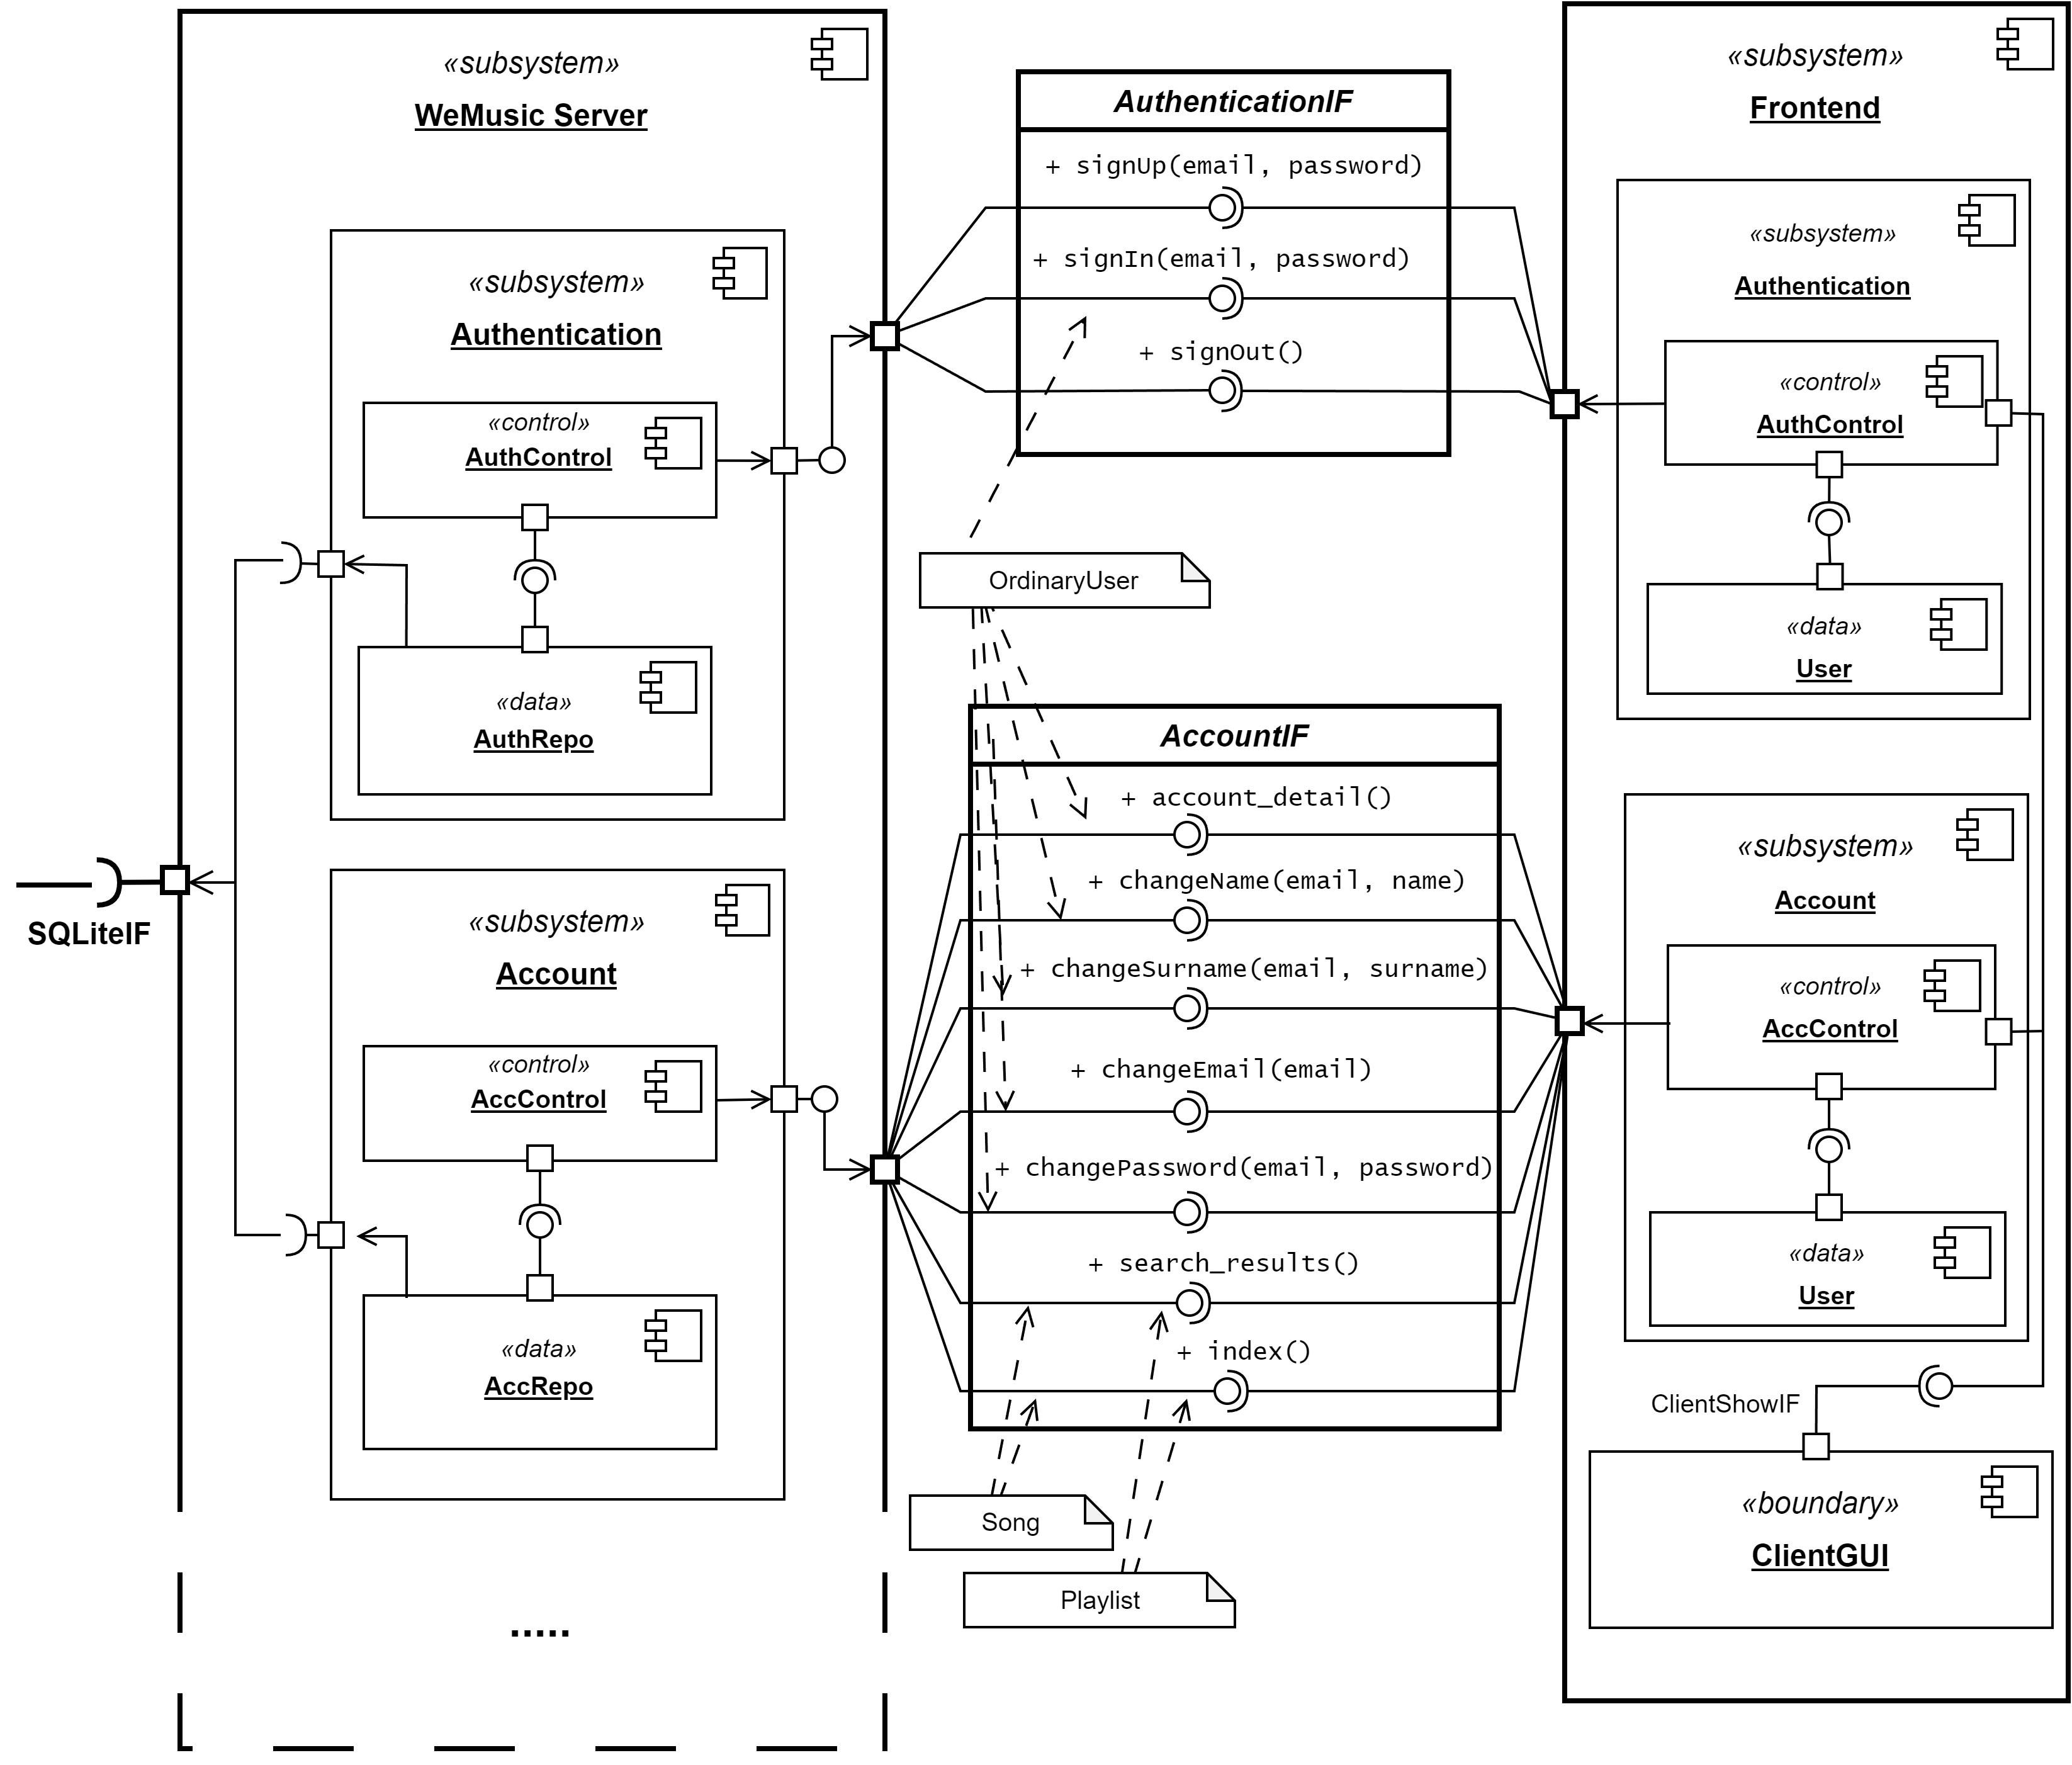
\includegraphics[scale=0.64]{component_diagram_ver4_3.png}
    \caption{UML Component Diagram}
    \label{fig-uml-component-diag_3}
\end{figure}

\newpage
\subparagraph{Musica}  In figura sono presenti tutte le interfacce
relative alla componente Musica, che include i brani, le playlist e gli album.
\begin{figure}[H]
    \centering
    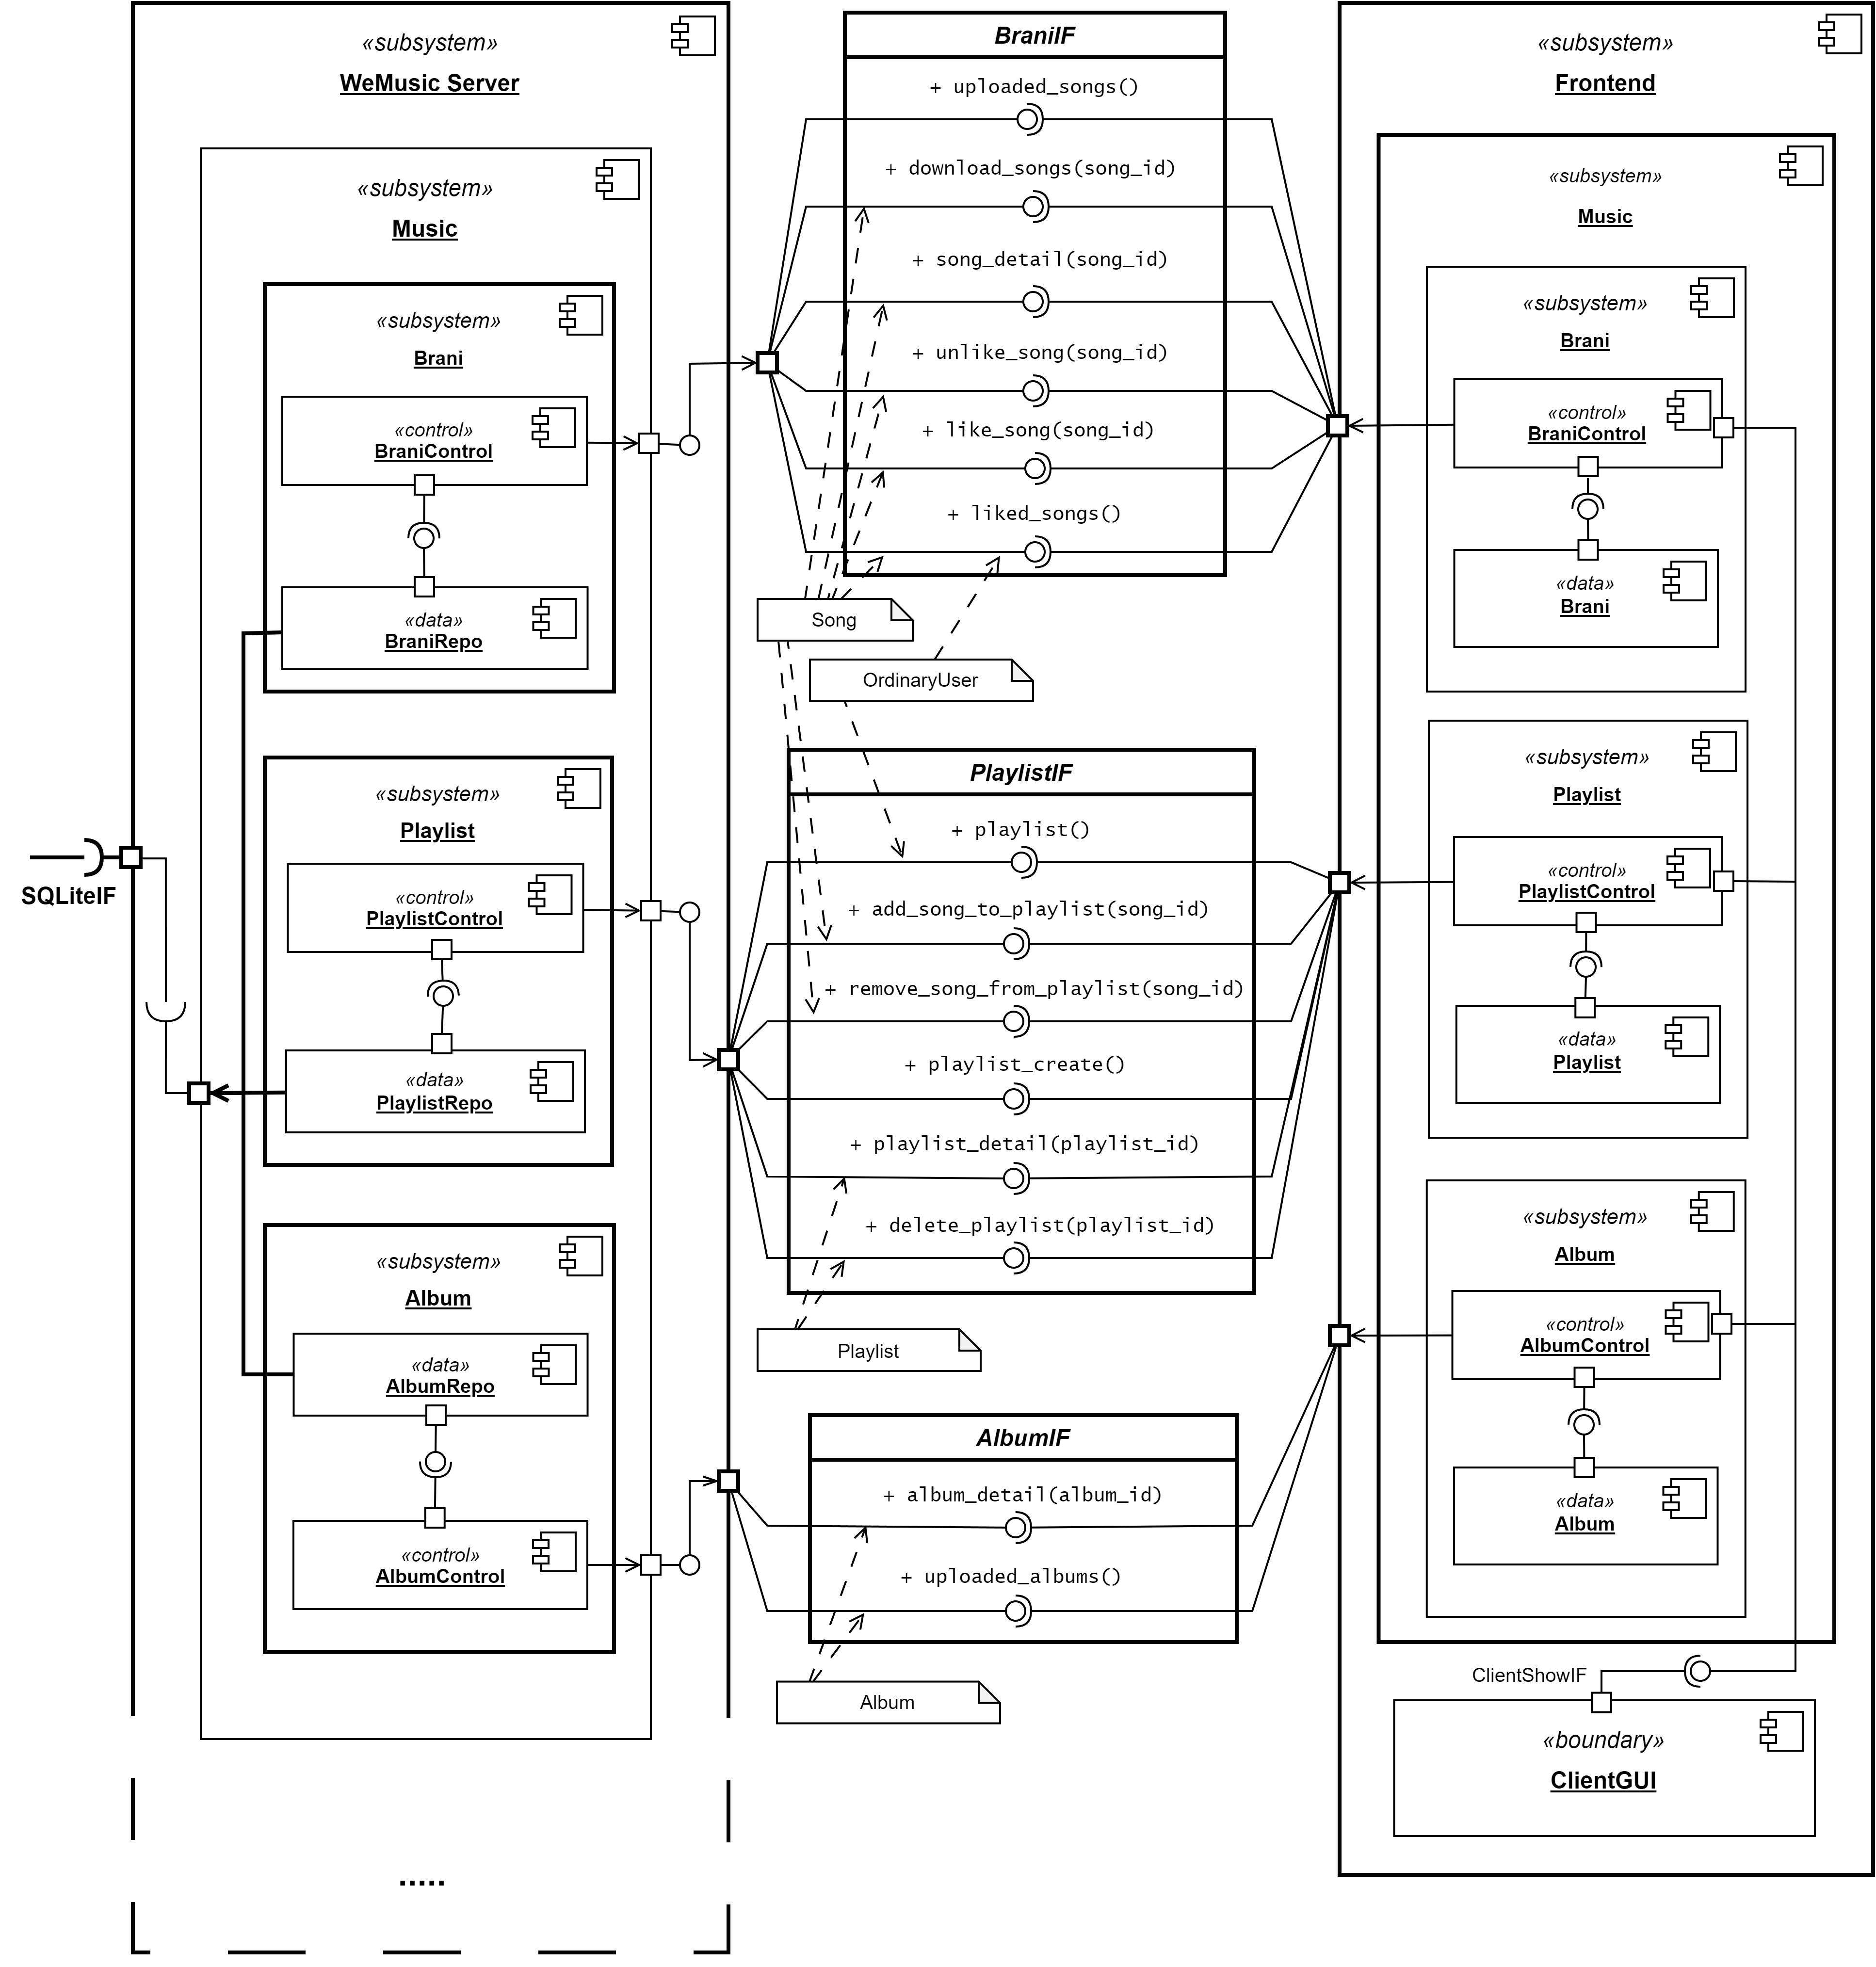
\includegraphics[scale=0.53]{component_diagram_ver4_4.png}
    \caption{UML Component Diagram}
    \label{fig-uml-component-diag_4}
\end{figure}

